\documentclass{sbmlpkgspec}
%\documentclass[draftspec]{sbmlpkgspec}

\usepackage{hyperref}
%\frontNotice{\centering This is a release candidate of the specification for the COMBINE archive and not a normative document. Please send feedback to the COMBINE mailing list at combine-archive@googlegroups.com.}

\usepackage{natbib}

\usepackage{url}

\begin{document}

\packageGeneralURL{http://co.mbine.org/documents/archive}
\packageTitle{COMBINE Archive Specification}
\packageVersion{Version 1} \packageVersionDate{\today}
\packageThisVersionURL{http://co.mbine.org/documents/archive}

\author{%
\begin{tabular}{c>{\hspace{20pt}}c}
Frank T. Bergmann & Nicolas Rodriguez \\[0.25em]
\mailto{fbergmann@caltech.edu} & \mailto{rodriguezn@babraham.ac.uk}\\[0.25em]
Computing and Mathematical Sciences & Babraham Institute\\
California Institute of Technology & Babraham Campus Cambridge\\
Pasadena, CA, US & Cambridge, UK\\
\\
Nicolas Le Nov\`{e}re\\[0.25em]
\mailto{n.lenovere@gmail.com}\\[0.25em]
Babraham Institute\\
Babraham Campus Cambridge\\
Cambridge, UK\\
\end{tabular}
}

\renewcommand\graphicspath{{logos}}

\newcommand{\OmexManifest}{\defRef{OmexManifest}{manifest-class}\xspace}
\newcommand{\Content}{\defRef{Content}{content-class}\xspace}
\newcommand{\sbmlthreecore}{SBML Level~3 Version~1 Core\xspace}

\maketitlepage
\maketableofcontents

\section{Document conventions} \label{conventions} 

Following the precedent set by other COMBINE specification
documents, we use UML~1.0 (Unified Modeling Language; 
\citet{eriksson:1998,oestereich:1999}) class diagram notation to 
define the constructs provided by this package. 

We also use the following typographical conventions to distinguish the 
names of objects and data types from other entities: 

\begin{description} 

\item \class{Class}: Names of ordinary (concrete) classes begin with a 
capital letter and are printed in an upright, bold, sans-serif typeface. 
In electronic document formats, the class names are also hyperlinked to 
their definitions in this specification document. 

\item \token{SomeThing}, \token{otherThing}: Attributes of classes, data 
type names, literal XML, and generally all tokens \emph{other} than 
UML class names, are printed in an upright typewriter typeface. 
Primitive types defined begin with a capital letter; the COMBINE archive
also makes use of primitive types defined by XML 
Schema~1.0~\citep{biron:2000,fallside:2000,thompson:2000}, but 
unfortunately, XML~Schema does not follow any capitalization convention 
and primitive types drawn from the XML~Schema language may or may not 
start with a capital letter. 

\end{description} 
 
% -*- TeX-master: "main"; fill-column: 72 -*-

\section{Background}  \label{background} 

\subsection{Motivation}

Computational modeling is an increasingly interdisciplinary field. Different aspects of the modeling activity come together, that need information to be stored in a cohesive unit. When sharing a model, not exchanging all relevant files might cause problems. Several different approaches have been tried to solve this issue, such as folder based project structures, or special versions of version control systems. Unfortunately these approaches are not as easy to support for tool authors as a single file based solution would. 

This specification describes \textit{COMBINE archive}, a file that contains all the information needed to describe a modeling and simulation experiment. The \textit{COMBINE archive} is encoded with the \emph{Open Modeling Exchange format} (OMEX).A \textit{COMBINE archive} is a single file containing the various documents (and possibly in the future, references to documents), necessary for the description of a model and all associated data and procedures. This includes for instance, but not limited to, simulation experiment descriptions in SED-ML, all models needed to run the simulations in SBML or CellML
and their graphical representations in SBGN-ML. 

The COMBINE archive aims to augment these efforts by standardizing a manifest that describes all files in the archive, guidance for encoding metadata and a convention for bundling the information together. Such an approach also allow resources using a distributed version control system (such as PMR2, \url{http://models.cellml.org/}) to export COMBINE archives, by generating a manifest file during export. 
http://models.cellml.org/
Details of earlier independent proposals are provided below. 

\subsection{History}

The COMBINE Archive was engendered from the SED-ML Archive, that was first introduced in the SED-ML mailing list in 2009, and briefly described in SED-ML Level~1 Version~1 \citep{Waltemath:2011}. The SED-ML Archive addressed the need of providing a way to include all relevant models used in a SED-ML simulation experiment along with the experiment specification. The SED-ML archive is basically the convention to provide, inside a ZIP file (with extension .sedx), a SED-ML document with the same base name as the archive and all models listed in the SED-ML file. 

This specification has been created out of the many discussions that took place
on the combine-discuss mailing list. The primary threads are located here: 

\begin{itemize}
	\item \href{http://listserver.ebi.ac.uk/pipermail/combine-discuss/2011-October/thread.html}{http://listserver.ebi.ac.uk/pipermail/combine-discuss/2011-October/thread.html}
	\item \href{http://listserver.ebi.ac.uk/pipermail/combine-discuss/2011-November/000016.html}{http://listserver.ebi.ac.uk/pipermail/combine-discuss/2011-November/000016.html}
	\item \href{http://listserver.ebi.ac.uk/pipermail/combine-discuss/2012-January/thread.html}{http://listserver.ebi.ac.uk/pipermail/combine-discuss/2012-January/thread.html}
\end{itemize}

The discussion continued at the last Hackathons, HARMONY 2012 where for the first time a larger audience discussed a preliminary proposal put together by Richard Adams, Frank T. Bergmann and Nicolas Le Nov\`{e}re \citep{Adams:2012}.  
Further discussions were held at HARMONY 2013.\\ (\url{https://docs.google.com/document/d/1ji2mOiWzXXl9ON6sU6Svd3E_IufowUCz24hklqci0iM/edit}). 

Discussions about the development of OMEX and the COMBINE archive are now taking place on the combine-archive Google group (\url{https://groups.google.com/forum/?#!forum/combine-archive}).

% -*- TeX-master: "main"; fill-column: 72 -*-

\section{Proposed syntax and semantics}
\label{syntax}

In this section, we define the syntax and semantics of the COMBINE 
Archive. We expound on the various data types and constructs defined, 
then in \sect{examples}, we provide complete examples of using the 
constructs in an example archive. 



\subsection{The archive format}
The COMBINE archive is a "zip" file \cite{zipFile}. Zip is a file format 
used for data compression and archiving. A zip file contains one or more 
files that have been compressed, to reduce file size, or stored as is. 
The technical specification of the ZIP format is available from the 
PKWARE website \cite{zipSpec}. 


\subsection{COMBINE archive extensions}
\label{combine-archive-extensions}
The extension for the COMBINE archive is \token{.omex}, for "{O}pen 
{M}odeling {EX}change format". 


Additional extensions indicate which standard formats are used within 
the archive, and help users to select appropriate software tools and 
in particular parsers. 
The extensions in use are: 


\begin{itemize}
	\item {\token{.sedx} - SED-ML archive} \cite{sedmll1v1}
	\item {\token{.sbex} - SBML archive} \cite{sbml}
	\item {\token{.cmex} - CellML archive} \cite{cellml11}
	\item {\token{.neux} - NeuroML archive} \cite{Gleeson2010}
	\item {\token{.phex} - PharmML archive} \cite{pharmml}
        \item {\token{.sbox} - SBOL archive} \cite{sbol}
\end{itemize}


\subsection{Content of the archive}

The archive contains: 

\begin{enumerate}
	\item {
	
     a mandatory manifest file, called \token{manifest.xml}, always located at the 
     root of the archive, that describes the location and the type of each 
     data files contained in the archive (including a special entry that represent
     the whole archive).
     
     The location of those files is defined by a relative path. In the current 
     version of the COMBINE archive, all the files described must be included 
     in the archive itself. It is envisioned that in the future the manifest 
     could list files located elsewhere, using valid and resolvable http 
     URIs. 

	}
	\item {
     a metadata file, called \token{metadata.*} (where \token{*} means the 
     suitable file extension) containing clerical information about the 
     various files contained in the archive, and the archive itself. 
	}
	\item {all the remaining files necessary to the model and simulation project. }

\end{enumerate}

\subsection{Namespace URI and other declarations necessary}
\label{xml-namespace}

The COMBINE archive defines two namespace URIs that allows to uniquely 
identify the manifest file and the whole archive.

The namespace URI for this version of OMEX is the following: 

\begin{center}
\uri{http://identifiers.org/combine.specifications/omex}
\end{center}

The namespace URI for this version of the COMBINE archive manifest is the following: 

\begin{center}
\uri{http://identifiers.org/combine.specifications/omex-manifest}
\end{center}



\subsection{Primitive data types}
\label{primtypes}

The COMBINE archive uses the XML Schema 1.0 data types~\citep{biron:2000}.
More specifically we make use of \primtype{string}.


\subsection{The \token{manifest.xml} file and the \class{OmexManifest} class}
\label{manifest-class}

At the root of the COMBINE archive stands one file, with the prescribed name \token{manifest.xml}. This file contains an instantiation of the \OmexManifest class. 

It contains a number of \Content children, one of which represents the COMBINE archive itself. 

Note that a valid manifest needs to have at least one entry, that of the whole archive, but may 
contain as many entries as needed. All the files in the archive should be listed in the manifest, the only
entry that is optionnal is the entry for the manifest.xml file as you are already reading its content.

\begin{figure}[h!]
  \centering
  % Requires \usepackage{graphicx}
  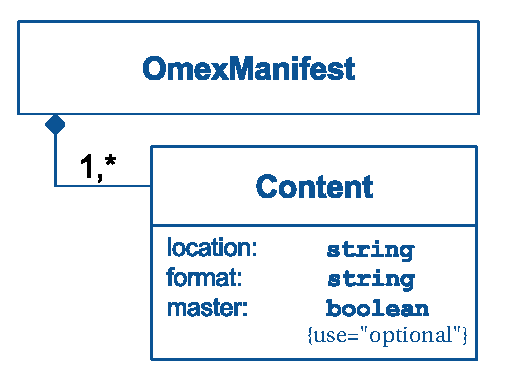
\includegraphics[width=6cm]{images/OmexManifest.pdf}\\
  \caption{A UML representation of the Manifest. Each manifest contains a number
	of Content elements.}
  \label{fig:combine_uml}
\end{figure}

\subsection{The \class{Content} class}
\label{content-class}
The \Content class represents an entry in the \OmexManifest and by 
extension a file in the \textit{COMBINE archive}. It consists of two 
required attributes: \token{location} and \token{format} and the 
optional attribute \token{master} 

\paragraph{The \token{location} attribute}
The \token{location} attribute is a required attribute of type 
\token{string}. It represents a relative location to an entry within the 
archive. The archive is represented by a dot \token{'.'}. 

\paragraph{The \token{format} attribute}
The \token{format} attribute is a required attribute of type \token{string}. It 
indicates the file type of the \Content element. The allowed values of the 
\token{format} attribute fall in two categories. Either the format 
denotes one of the COMBINE standards, in which case the \token{format} 
must begin with its \token{identifiers.org} URI. Or the 
\token{format} represents a Media type \cite{rfc2046}, in which case the \token{format} 
indicates the file type.

Using \token{identifiers.org} URI allows to unambiguously define the COMBINE standard, and even its level and version. For example, the identifier: \token{http://identifiers.org/combine.specifications/sbml} would denote the \Content 
element as being encoded in the SBML format. That is usually sufficient, as tools supporting one level of SBML usually
support others as well. However, if the software exporting the COMBINE archive wanted to be more precise, it could specify that it is an SBML Level 2 document with 

\begin{center}
\token{http://identifiers.org/combine.specifications/sbml.level-2}
\end{center}

or even declare its Version with 

\begin{center}
\token{http://identifiers.org/combine.specifications/sbml.level-2.version-3}.
\end{center}


The Media type \token{purl.org} URI should be of the form \token{http://purl.org/NET/mediatypes/}
followed by the MIME type. Here are a few examples :

\begin{example}
    for png (Portable Network Graphics) http://purl.org/NET/mediatypes/image/png
    for pdf (Portable Document Format) http://purl.org/NET/mediatypes/application/pdf
    for sbml http://purl.org/NET/mediatypes/application/sbml+xml
\end{example}

If both an \token{identifiers.org} URI and a MIME type are available for one specific format, the
\token{identifiers.org} URI must be used. 

%%TODO re-phrase
For compatibility reason, when reading a manifest.xml, you should be able to read format
attribute that contain only the MIME type, not in it's URI form. That is due to the fact that the draft specification
was allowing to use directly the MIME type for some time and some COMBINE archive using this form could be encountered.
However, when creating a new COMBINE archive, the URI form should always be used for MIME type.

\paragraph{The \token{master} attribute}
\label{active_document}
The \token{master} attribute is an optional attribute of type \token{boolean}. It 
represents a hint, that a certain file is to be used first when 
processing the content of an archive. Are top model description in a 
composed model, calling the various submodels; simulation description, 
calling the different model descriptions and data sources used in the 
experiment. In most cases, one content element per archive will have its \token{master} 
attribute set to \token{true}.

For example in the snippet below, it is the 
SED-ML element with \token{location="simulation.xml"} that a software 
program should first present to their users.

\begin{example}
<?xml version="1.0" encoding="utf-8"?>
<omexManifest xmlns="http://identifiers.org/combine.specifications/omex-manifest">
    <content location="." format="http://identifiers.org/combine.specifications/omex"/>
    <content location="manifest.xml" 
        format="http://identifiers.org/combine.specifications/omex-manifest"/>
    <content location="model/model.xml" format="http://identifiers.org/combine.specifications/sbml"/>
    <content location="simulation.xml" master="true"
        format="http://identifiers.org/combine.specifications/sed-ml"/>
    <content location="article.pdf" format="http://purl.org/NET/mediatypes/application/pdf"/>
    <content location="metadata.rdf"
        format="http://identifiers.org/combine.specifications/omex-metadata"/>
    <content location="diagram.sbgn" format="http://identifiers.org/combine.specifications/sbgn"/>
</omexManifest>
\end{example}

To simplify the identification, by a user or software, of the active document inside an archive, the file extensions 
(see also \ref{combine-archive-extensions}) can also be used. For the example above, 
where a SED-ML document is being marked as the master document, the 
recommended extension would be \token{.sbex}, to indicate that the software reading the archive need
to support the \token{SBML} format to be able to interpret the content of the archive. If the software
does support SED-ML as well as SBML, it should load the SED-ML file as the creator of the archive indicated
it to be the '\token{master}' file. If the software doesn't support SED-ML, it can still open the SBML document, ignoring
the master attribute.

Alternatively, if a software doesn't support either SBML or SED-ML but can open one of the other files, like the pdf
or diagram describing the model, it can choose to disregard the \token{master} attribute and the archive extension to present to the user the
files that it support.

In some cases, the \token{master} attribute could appear to be a duplication of the information given by the archive file
extension. But in other cases, like the example below, the \token{master} attribute add some usefull information.


\begin{example}
<?xml version="1.0" encoding="utf-8"?>
<omexManifest xmlns="http://identifiers.org/combine.specifications/omex-manifest">
    <content location="." format="http://identifiers.org/combine.specifications/omex"/>
    <content location="manifest.xml" 
        format="http://identifiers.org/combine.specifications/omex-manifest"/>
    <content location="main-model.xml" master="true"
        format="http://identifiers.org/combine.specifications/cellml.1.1"/>
    <content location="submodel1.xml" 
        format="http://identifiers.org/combine.specifications/cellml.1.1"/>
    <content location="submodel2.xml" 
        format="http://identifiers.org/combine.specifications/cellml.1.1"/>
    <content location="article.pdf" format="http://purl.org/NET/mediatypes/application/pdf"/>
    <content location="metadata.rdf"
        format="http://identifiers.org/combine.specifications/omex-metadata"/>
</omexManifest>
\end{example}

The archive, described by this manifest.xml, contain a modular CellML model. Even if the extension of the archive is \token{cmex}, it
does not help knowing which file to open first since there are several CellML files. The \token{master} attribute allow the software
to know which file encode the whole model.

Most archives will concern only one model and should have only one \token{master} attribute set to \token{true}. Although in some cases, the creator of the archive might want to set several \token{master} attribute to \token{true}, may be to indicate alternative renditions of a model if they have different \token{format}, may be to indicate different models that are part of the same experiment or publication. Then the reading software are free to open a given one, all of them or display a dialog box to the user so that he can chose the one(s) he want to open. This might create some confusion as opening the same archive several times in the same software might result in a different model loaded. One option, for those more complex archives, would be to not have any \token{master} attribute set to \token{true} but it might be difficult when an archive contain many files, in particular modular models.


\subsection{Advised format for the archive metadata}

One can include any type of file in a COMBINE archive, and therefore any 
type of metadata format. However, in the interest of interoperability, 
and to ease the development of software support for metadata, a 
recommended format is provided as part of the specification of the 
archive. 

The recommended format is based on several standards developed by other 
organisations: 

\begin{itemize}
	\item  {
	
     The \href{http://www.w3.org/RDF/ }{ Resource Description Format} of the 
     W3C, in particular its terms:
     \begin{itemize}
		\item \token{RDF}, 
		\item \token{Description}, 
		\item \token{Bag}, 
		\item \token{li}.
	\end{itemize}
	}
	\item  {

	vCard 4 (\cite{rfc6350}), a file format standard for electronic business 
    cards, in particular its terms:
    	\begin{itemize}
		\item \token{hasName}, 
		\item \token{family-name}, 
		\item \token{given-name}, 
		\item \token{hasEmail},
		\item \token{organization-name}.
	\end{itemize}

	More information on how to use vCard in RDF can be found 
    on the W3C website\footnote[1]{\url{http://www.w3.org/TR/vcard-rdf/ }}.
	
	}
	\item {
	
	Metadata terms\footnote[2]{\url{http://dublincore.org/documents/dcmi-terms/}} of 
	the Dublin Core Metadata Initiative, in particular the terms: 

	\begin{itemize}
		\item \token{description}, 
		\item \token{creator}, 
		\item \token{created}, 
		\item \token{modified},
		\item \token{W3CDTF}.
	\end{itemize}
		
	More information on the use of Dublin Core in RDF can be found 
	on the Dublin Core website{\footnote[3]{\url{http://dublincore.org/documents/dc-rdf/}}}. } 
	
	More information is available about the definition of the date format used within \token{dcterms:created} and 
	\token{dcterms:modified} elements{\footnote[4]{\url{http://www.w3.org/TR/NOTE-datetime}}}.

\end{itemize}

Users of the COMBINE standards may already be familiar with this 
approach, as it is also taken by SBML, SED-ML, SBGN-ML. 
Note however that the format here slightly differs from the controlled 
annotations of SBML. The differences have been made to address inconsistencies 
in the SBML vCard specification and to follow W3C recommendations {\footnote[4]{\url{http://www.w3.org/TR/vcard-rdf/}}} . The changes 
are:

\begin{itemize}
	\item  "n" becomes "hasName" 
	\item  "Family" becomes "family-name" 
	\item  "Given" becomes "given-name" 
	\item  "EMAIL" becomes "hasEmail" 
	\item  "Orgname" becomes "organization-name" 
\end{itemize}

A \textit{COMBINE archive} can include multiple metadata elements. To 
identify that a particular \Content element is being annotated, the 
\token{rdf:about} attribute should use the same value that is also used 
in \token{location} of the \Content element. 


\begin{example}
<?xml version="1.0" encoding="UTF-8"?>
<rdf:RDF xmlns:rdf="http://www.w3.org/1999/02/22-rdf-syntax-ns#" 
         xmlns:dcterms="http://purl.org/dc/terms/" 
				 xmlns:vCard="http://www.w3.org/2006/vcard/ns#">
   <rdf:Description rdf:about="./simulation.xml">
   ...
	 </rdf:Description>
</rdf:RDF>
\end{example}

The example above signifies that a content element with 
\token{location="./simulation.xml"} is described. A complete example of 
the metadata related to a simulation description contained in a COMBINE 
archive is described in \ref{examples}. 



% -*- TeX-master: "main"; fill-column: 72 -*-

\section{Illustrative examples of the syntax}
\label{examples}

This section contains a worked example showing the encoding of a model 
and associated data in a COMBINE archive. First the \OmexManifest, that 
includes five entries. One of these entries is the \OmexManifest itself, 
it has a fixed location \token{location="./manifest.xml"}. Additionally 
the archive includes an SBML model, a SED-ML description. It also 
includes a PDF file that is specified through its MIME type. Finally 
associated meta information for clerical data is included in 
\token{location="./metadata.rdf"}. 


\begin{example}
<?xml version="1.0" encoding="utf-8"?>
<omexManifest xmlns="http://identifiers.org/combine.specifications/omex-manifest">
    <content location="." 
		         format="http://identifiers.org/combine.specifications/omex"/>
    <content location="./manifest.xml" 
		         format="http://identifiers.org/combine.specifications/omex-manifest"/>
    <content location="./model/model.xml" 
		         format="http://identifiers.org/combine.specifications/sbml"/>
    <content location="./simulation.xml" 
		         format="http://identifiers.org/combine.specifications/sedml"/>
    <content location="./article.pdf" 
		         format="application/pdf"/>
    <content location="./metadata.rdf" 
		         format="http://identifiers.org/combine.specifications/omex-metadata"/>
</omexManifest>
\end{example}

Here a complete example, on how the clerical data could be encoded: 

\begin{example}
<?xml version="1.0" encoding="UTF-8"?>
<rdf:RDF xmlns:rdf="http://www.w3.org/1999/02/22-rdf-syntax-ns#" 
         xmlns:dcterms="http://purl.org/dc/terms/" 
				 xmlns:vCard="http://www.w3.org/2006/vcard/ns#">

   <rdf:Description rdf:about="./simulation.xml">
      <dcterms:description>SED-ML Description Representing a 1D Steady Scan 
			   experiment carried out on the Heinrich Oscillator model. 
			</dcterms:description>
      <dcterms:creator>
         <rdf:Bag>
            <rdf:li rdf:parseType="Resource">
               <vCard:hasName rdf:parseType="Resource">
                  <vCard:family-name>Bergmann</vCard:family-name>
                  <vCard:given-name>Frank</vCard:given-name>
               </vCard:hasName>
               <vCard:hasEmail rdf:resource="fbergman@caltech.edu">
               <vCard:organization-name>
		      California Institute of Technology
	       </vCard:organization-name>
            </rdf:li>
         </rdf:Bag>
      </dcterms:creator>
      <dcterms:created rdf:parseType="Resource">
         <dcterms:W3CDTF>2014-01-20T19:52:11Z</dcterms:W3CDTF>
      </dcterms:created>
      <dcterms:modified rdf:parseType="Resource">
         <dcterms:W3CDTF>2014-01-20T19:54:05Z</dcterms:W3CDTF>
      </dcterms:modified>
   </rdf:Description>
</rdf:RDF>
\end{example}

% -*- TeX-master: "main"; fill-column: 72 -*-

\section{Best practices}
\label{best-practices}

In this section, we recommend a number of practices for using and 
interpreting various constructs in the COMBINE Archive. These 
recommendations are non-normative, but we advocate them strongly; 
ignoring them will not render a model invalid, but may reduce 
inter-operability between software and models. 


% -*- TeX-master: "main"; fill-column: 72 -*-

\section{Future development}
\label{future}
In this section we highlight some open issues not addressed in this 
version of the COMBINE archive specification. 


\subsection{Linking to external documents}
It was often discussed to also allow the \token{location} elements of a 
\Content element point to an external document. However, in this first 
version we restrict them to local files, so as to make it easier to 
adopt in software tools. That way tools could focus on the primary use 
case of bundling up several local resources, rather than worry about 
retrieving information from online resources that may not always be 
available or may be more complex.

\subsection{Cross References between entries}
At HARMONY we spend some time discussing whether cross references 
between the individual entries in the archive ought to be in this first 
version of the specification. However, it was decided to leave the cross 
referencing to the individual standards for now, rather to impose them 
ad-hoc. 

\subsection{Alternative versions of the archive metadata}
It was suggested to allow different versions of the archive metadata 
format. The manifest already provides a way for referencing alternate 
versions, all that would need to be changed, would be the format 
identifier to point to a different specification rather than: 


\url{http://identifiers.org/combine.specifications/omex-metadata}

However, as of the time of this writing no such format was proposed.

% and finally the appendix and end stuff

\setcounter{secnumdepth}{2}
\appendix
%% -*- TeX-master: "main"; fill-column: 72 -*-
\section{Validation of SBML documents} \label{apdx-validation}

\subsection{Validation and consistency rules} \label{validation-rules}

This section summarizes all the conditions that must (or in some cases,
at least \emph{should}) be true of an SBML Level~3 Version~1 model that
uses the \FBCPackage. We use the same conventions as are used in the
SBML Level~3 Version~1 Core specification document. In particular, there
are different degrees of rule strictness. Formally, the differences are
expressed in the statement of a rule: either a rule states that a
condition \emph{must} be true, or a rule states that it \emph{should} be
true. Rules of the former kind are strict SBML validation rules---a
model encoded in SBML must conform to all of them in order to be
considered valid. Rules of the latter kind are consistency rules. To
help highlight these differences, we use the following three symbols
next to the rule numbers:

\begin{description}

\item[\hspace*{6.5pt}\vSymbol\vsp] A \vSymbolName indicates a
\emph{requirement} for SBML conformance. If a model does not follow this
rule, it does not conform to the Flux Balance Constraints specification.
(Mnemonic intention behind the choice of symbol: ``This must be
checked.'')

\item[\hspace*{6.5pt}\cSymbol\csp] A \cSymbolName indicates a
\emph{recommendation} for model consistency. If a model does not follow
this rule, it is not considered strictly invalid as far as the Flux
Balance Constraints specification is concerned; however, it indicates
that the model contains a physical or conceptual inconsistency.
(Mnemonic intention behind the choice of symbol: ``This is a cause for
warning.'')

\item[\hspace*{6.5pt}\mSymbol\msp] A \mSymbolName indicates a strong
recommendation for good modeling practice. This rule is not strictly a
matter of SBML encoding, but the recommendation comes from logical
reasoning. As in the previous case, if a model does not follow this
rule, it is not strictly considered an invalid SBML encoding. (Mnemonic
intention behind the choice of symbol: ``You're a star if you heed
this.'')

\end{description}

The validation rules listed in the following subsections are all stated
or implied in the rest of this specification document. They are
enumerated here for convenience. Unless explicitly stated, all
validation rules concern objects and attributes specifically defined in
the Flux Balance Constraints package.

For \notice convenience and brevity, we use the shorthand
``\token{fbc:\-x}'' to stand for an attribute or element name \token{x}
in the namespace for the \FBCPackage, using the namespace prefix
\token{fbc}. In reality, the prefix string may be different from the
literal ``\token{fbc}'' used here (and indeed, it can be any valid XML
namespace prefix that the modeler or software chooses). We use
``\token{fbc:\-x}'' because it is shorter than to write a full
explanation everywhere we refer to an attribute or element in the
\FBCPackage namespace.

\subsubsection*{General rules about this package}

\validRule{fbc-10101}{To conform to the \FBCPackage specification for
SBML Level~3 Version~1, an SBML document must declare the use of the
following XML Namespace:\\
\textsl[-25]{\uri{http://www.sbml.org/sbml/level3/version1/fbc/version1}
}. (References: SBML Level~3 Package Specification for Flux Balance
Constraints, Version~1, \sec{xml-namespace}.)}

\validRule{fbc-10102}{Wherever they appear in an SBML document, elements
and attributes from the \FBCPackage must be declared either implicitly
or explicitly to be in the XML namespace
\uri{http://www.sbml.org/sbml/level3/version1/fbc/version1}.
(References: SBML Level~3 Package Specification for Flux Balance
Constraints , Version~1, \sec{xml-namespace}.) }

\subsubsection*{General rules about identifiers}

\validRule{fbc-10301}{(Extends validation rule \#10301 in the SBML
Level~3 Version~1 Core specification.) Within a \Model the values of the
attributes \token{id} and \token{fbc:\-id} on every instance of the
following classes of objects must be unique across the set of all
\token{id} and \token{fbc:\-id} attribute values of all such objects in
a model: the \Model itself, plus all contained \FunctionDefinition,
\Compartment, \Species, \Reaction, \SpeciesReference,
\ModifierSpeciesReference, \Event, and \Parameter objects, plus the
\FluxBound, \Objective and \FluxObjective objects defined by the
\FBCPackage. (References: SBML Level~3 Package Specification for Flux
Balance Constraints, Version~1, \sec{primtypes}.) }

\validRule{fbc-10302} {
The value of a \token{fbc:\-id} attribute must always conform to the
syntax of the SBML data type \primtype{SId}. (References: SBML Level~3
Package Specification for Flux Balance Constraints, Version~1,
\sec{primtypes}.)
}

\subsubsection*{Rules for the extended \class{SBML} class}

\validRule{fbc-20101}{In all SBML documents using the \FBCPackage, the
\SBML object must include a value for the attribute
\token{fbc:\-required} attribute. (References: SBML Level~3 Version~1
Core, Section~4.1.2.) }

\validRule{fbc-20102}{The value of attribute \token{fbc:\-required} on
the \SBML object must be of the data type \primtype{boolean}.
(References: SBML Level~3 Version~1 Core, Section~4.1.2.) }

\validRule{fbc-20103}{The value of attribute \token{fbc:\-required} on
the \SBML object must be set to \val{false}. (References: SBML Level~3
Package Specification for Flux Balance Constraints, Version~1,
\sec{xml-namespace}.) }

\subsubsection*{Rules for extended \class{Model} object}

\validRule{fbc-20201}{There may be at most one instance of each of the
following kinds of objects within a \Model object using Flux Balance
Constraints: \ListOfFluxBounds and \ListOfObjectives. (References: SBML
Level~3 Package Specification for Flux Balance Constraints, Version~1,
\sec{model-class}.) }

\validRule{fbc-20202}{The various
\textsf{\textbf{ListOf\rule{0.15in}{0.5pt}}} subobjects with an \Model
object are optional, but if present, these container object must not
be empty. Specifically, if any of the following classes of objects are
present on the \Model, it must not be empty: \ListOfFluxBounds and
\ListOfObjectives. (References: SBML Level~3 Package Specification for
Flux Balance Constraints, Version~1, \sec{model-class}.) }

\validRule{fbc-20203}{Apart from the general notes and annotation
subobjects permitted on all SBML objects, a \ListOfFluxBounds container
object may only contain \FluxBound objects. (References: SBML Level~3
Package Specification for Flux Balance Constraints, Version~1,
\sec{model-class}.) }

\validRule{fbc-20204}{Apart from the general notes and annotation
subobjects permitted on all SBML objects, a \ListOfObjectives container
object may only contain \Objective objects. (References: SBML Level~3
Package Specification for Flux Balance Constraints, Version~1,
\sec{model-class}.) }

\validRule{fbc-20205}{A \ListOfFluxBounds object may have the optional
attributes \token{meta\-id} and \token{sboTerm} defined by SBML Level~3
Core. No other attributes from the SBML Level~3 Core namespace or the
Flux Balance Constraints namespace are permitted on a \ListOfFluxBounds
object. (References: SBML Level~3 Package Specification for Flux Balance
Constraints, Version~1, \sec{model-class}.) }

\validRule{fbc-20206}{A \ListOfObjectives object may have the optional
attributes \token{meta\-id} and \token{sboTerm} defined by SBML Level~3
Core. Additionally the \ListOfObjectives must contain the attribute
\token{active\-Objective}. No other attributes from the SBML Level~3
Core namespace or the Flux Balance Constraints namespace are permitted
on a \ListOfObjectives object. (References: SBML Level~3 Package
Specification for Flux Balance Constraints, Version~1,
\sec{model-class}.) }

\validRule{fbc-20207}{The value of attribute
\token{fbc:\-activeObjective} on the \ListOfObjectives object must be of
the data type \primtype{SIdRef}. (References: SBML Level~3 Package
Specification for Flux Balance Constraints, Version~1,
\sec{activeObjective-attribute}). }

\validRule{fbc-20208}{The value of attribute
\token{fbc:\-activeObjective} on the \ListOfObjectives object must be
the identifier of an existing \Objective. (References: SBML Level~3
Package Specification for Flux Balance Constraints, Version~1,
\sec{activeObjective-attribute}.) }

\subsubsection*{Rules for extended \class{Species} object}

\validRule{fbc-20301}{A \SBML \class{Species} object may have the
optional attributes \token{fbc:\-charge} and
\token{fbc:\-chemicalFormula}. No other attributes from the Flux Balance
Constraints namespaces are permitted on a \class{Species}. (References:
SBML Level~3 Package Specification for Flux Balance Constraints,
Version~1, \sec{species-class}) }

\validRule{fbc-20302}{The value of attribute \token{fbc:\-charge} on
the \SBML \class{Species} object must be of the data type
\primtype{integer}. (References: SBML Level~3 Package Specification for
Flux Balance Constraints, Version~1, \sec{species-class}). }

\validRule{fbc-20303}{The value of attribute
\token{fbc:\-chemicalFormula} on the \SBML \class{Species} object must
be set to a \primtype{string} consisting only of atomic names or user
defined compounds and their occurrence. (References: SBML Level~3 Package
Specification for Flux Balance Constraints, Version~1,
\sec{species-class}.) }

\subsubsection*{Rules for \class{FluxBound} object}

\validRule{fbc-20401}{A \FluxBound object may have the optional SBML
Level 3 Core attributes \token{metaid} and \token{sboTerm}. No other
attributes from the SBML Level 3 Core namespace are permitted on a
\FluxBound. (References: SBML Level~3 Version~1 Core, Section~3.2.) }

\validRule{fbc-20402}{A \FluxBound object may have the optional SBML
Level 3 Core subobjects for notes and annotations. No other elements
from the SBML Level 3 Core namespace are permitted on a \FluxBound.
(References: SBML Level~3 Version~1 Core, Section~3.2.) }

\validRule{fbc-20403}{A \FluxBound object must have the required
attributes \token{fbc:\-reaction}, \token{fbc:\-operation} and
\token{fbc:\-value}, and may have the optional attributes
\token{fbc:\-id} and \token{fbc:\-name}. No other attributes from the
SBML Level~3 Flux Balance Constraints namespace are permitted on a
\FluxBound object. (References: SBML Level~3 Package Specification for
Flux Balance Constraints, Version~1, \sec{fluxbound-class}.) }

\validRule{fbc-20404}{The attribute \token{fbc:\-reaction} of a \FluxBound
must be of the data type \token{SIdRef}. (References: SBML Level~3
Package Specification for Flux Balance Constraints, Version~1,
\sec{fluxbound-class}.) }

\validRule{fbc-20405}{The attribute \token{fbc:\-name} of a \FluxBound
must be of the data type \token{string}. (References: SBML Level~3
Package Specification for Flux Balance Constraints, Version~1,
\sec{fluxbound-class}.) }

\validRule{fbc-20406}{The attribute \token{fbc:\-operation} of a
\FluxBound must be of the data type \token{FbcOperation} and thus its
value must be one of \val{lessEqual}, \val{greaterEqual} or \val{equal}.
(References: SBML Level~3 Package Specification for Flux Balance
Constraints, Version~1, \sec{fluxbound-class}.) }

\validRule{fbc-20407}{The attribute \token{fbc:\-value} of a \FluxBound
must be of the data type \token{double}. (References: SBML Level~3
Package Specification for Flux Balance Constraints, Version~1,
\sec{fluxbound-class}.) }

\validRule{fbc-20408}{The value of the attribute \token{fbc:\-reaction}
of a \FluxBound object must be the identifier of an existing \Reaction
object defined in the enclosing \Model object. (References: SBML Level~3
Package Specification for Flux Balance Constraints, Version~1,
\sec{fluxbound-class}.) }

\validRule{fbc-20409}{The combined set of all \FluxBound's with
identical values for \token{fbc:\-reaction} must be consistent. That is
while it is possible to define a lower and an upper bound for a
reaction, it is not possible to define multiple lower or upper bounds.
(References: SBML Level~3 Package Specification for Flux Balance
Constraints, Version~1, \sec{fluxbound-class}.) }

\subsubsection*{Rules for \class{Objective} object}

\validRule{fbc-20501}{A \Objective object may have the optional SBML
Level 3 Core attributes \token{metaid} and \token{sboTerm}. No other
attributes from the SBML Level 3 Core namespace are permitted on a
\Objective. (References: SBML Level~3 Version~1 Core, Section~3.2.) }

\validRule{fbc-20502}{A \Objective object may have the optional SBML
Level 3 Core subobjects for notes and annotations. No other elements
from the SBML Level 3 Core namespace are permitted on a \Objective.
(References: SBML Level~3 Version~1 Core, Section~3.2.) }

\validRule{fbc-20503}{A \Objective object must have the required
attributes \token{fbc:\-id} and \token{fbc:\-type} and may have the
optional attribute \token{fbc:\-name}. No other attributes from the SBML
Level~3 Flux Balance Constraints namespace are permitted on a \Objective
object. (References: SBML Level~3 Package Specification for Flux Balance
Constraints, Version~1, \sec{objective-class}.) }

\validRule{fbc-20504}{The attribute \token{fbc:\-name} on a \Objective
must be of the data type \token{string}. (References: SBML Level~3
Package Specification for Flux Balance Constraints, Version~1,
\sec{objective-class}.) }

\validRule{fbc-20505}{The attribute \token{fbc:\-type} on a \Objective
must be of the data type \token{FbcType} and thus its value must be one
of \val{minimize} or \val{maximize}. (References: SBML Level~3
Package Specification for Flux Balance Constraints, Version~1,
\sec{objective-class}.) }

\validRule{fbc-20506}{A \Objective object must have one and only one
instance of the \ListOfFluxObjectives object. (References: SBML Level~3
Package Specification for Flux Balance Constraints, Version~1,
\sec{objective-class}.) }

\validRule{fbc-20507}{The \ListOfFluxObjectives subobject within a
\Objective object must not be empty. (References: SBML Level~3 Package
Specification for Flux Balance Constraints, Version~1,
\sec{objective-class}.) }

\validRule{fbc-20508}{Apart from the general notes and annotation
subobjects permitted on all SBML objects, a \ListOfFluxObjectives
container object may only contain \FluxObjective objects. (References: SBML
Level~3 Package Specification for Flux Balance Constraints, Version~1,
\sec{objective-class}.) }

\validRule{fbc-20509}{A \ListOfFluxObjectives object may have the
optional \token{meta\-id} and \token{sboTerm} defined by SBML Level~3
Core. No other attributes from the SBML Level~3 Core namespace or the
Flux Balance Constraints namespace are permitted on a
\ListOfFluxObjectives object. (References: SBML Level~3 Package
Specification for Flux Balance Constraints, Version~1,
\sec{objective-class}.) }

\subsubsection*{Rules for \class{FluxObjective} object}

\validRule{fbc-20601}{A \FluxObjective object may have the optional SBML
Level 3 Core attributes \token{metaid} and \token{sboTerm}. No other
attributes from the SBML Level 3 Core namespace are permitted on a
\FluxObjective. (References: SBML Level~3 Version~1 Core, Section~3.2.)
}

\validRule{fbc-20602}{A \FluxObjective object may have the optional SBML
Level 3 Core subobjects for notes and annotations. No other elements
from the SBML Level 3 Core namespace are permitted on a \FluxObjective.
(References: SBML Level~3 Version~1 Core, Section~3.2.) }

\validRule{fbc-20603}{A \FluxObjective object must have the required
attributes \token{fbc:\-reaction} and \token{fbc:\-coefficient}, and may
have the optional attributes \token{fbc:\-id} and \token{fbc:\-name}. No
other attributes from the SBML Level~3 Flux Balance Constraints
namespace are permitted on a \FluxObjective object. (References: SBML
Level~3 Package Specification for Flux Balance Constraints, Version~1,
\sec{fluxobjective-class}.) }

\validRule{fbc-20604}{The attribute \token{fbc:\-name} on a \FluxObjective
must be of the data type \token{string}. (References: SBML Level~3
Package Specification for Flux Balance Constraints, Version~1,
\sec{fluxobjective-class}.) }

\validRule{fbc-20605}{The value of the attribute \token{fbc:\-reaction}
of a \FluxObjective object must conform to the syntax of the SBML data
type \primtype{SIdRef}. (References: SBML Level~3 Package Specification
for Flux Balance Constraints, Version~1, \sec{fluxobjective-class}.) }

\validRule{fbc-20606}{The value of the attribute \token{fbc:\-reaction}
of a \FluxObjective object must be the identifier of an existing
\Reaction object defined in the enclosing \Model object. (References:
SBML Level~3 Package Specification for Flux Balance Constraints,
Version~1, \sec{fluxobjective-class}.) }

\validRule{fbc-20607}{The value of the attribute
\token{fbc:\-coefficient} of a \FluxObjective object must conform to the
syntax of the SBML data type \primtype{double}. (References: SBML
Level~3 Package Specification for Flux Balance Constraints, Version~1,
\sec{fluxobjective-class}.) }



\setcounter{secnumdepth}{-1}
% -*- TeX-master: "main"; fill-column: 72 -*-

\section{Acknowledgments}
We would like to thank all the people who contributed in various ways to the development of both the original proposal and this specification, especially Richard Adams and Stuart Moodie. 
We also would like to thank the attendees of dedicated sessions at COMBINE meetings and the members of the \textsf{combine-discuss} and \textsf{combine-archive} mailing lists and all others who contributed to 
discussions on various occasions. 






\clearpage
\bibliography{combine_archive}


\end{document}
